\section{Transformada de Laplace}

\begin{definition}
  La transformada de Laplace $\mathcal{L}[f(t)]$ de una función $F(s)$ definida por 
  \begin{equation}
    \mathcal{L}[f(s)](s) = \int_0^\infty e^{-st}dt
  \end{equation}
  para todo $s$ tal que esta integral converja.
\end{definition}

La transformada de Laplace convierte una función $f$ en una nueva llamada $\mathcal{L}[f(t)]$. Con frecuencia $t$ es la variable independiente para $f$ y $s$ es la variable independiente para $\mathcal{L}[f]$. Así, $f(t)$ es la función $f$ evaluada en $t$ y $\mathcal{L}[f](s)$ es la función $\mathcal{L}[f]$ evaluada en $s$.

Es necesario convenir en usar letras minúsculas para la función transformada de Laplace, y su letra mayúscula para la función que resulta. En notación 
$$
F = \mathcal{L}[f], \quad G = \mathcal{L}[g], \quad H = \mathcal{L}[h]
$$
y así sucesivamente.

\begin{example}
  Sea $f(t)=e^{at}$, siendo $a$ cualquier número real. Entonces
  \begin{align*}
    \mathcal{L}[f(t)] &= F(s) = \int_0^\infty e^{-st}e^{at}dt = \int_0^\infty e^{(a-s)t}dt \\ 
                        &= \lim_{k\to\infty}\int_0^k e^{(a-s)t}dt =\lim_{k\to\infty}\left[\frac{1}{a-s}e^{(a-s)t}\right\rvert_0^k \\ 
                        &= \lim_{k\to\infty} \frac{e^{(a-s)k}}{a-s} - \frac{\cancel{e^0}}{a-s} \\ 
                        &= \lim_{k\to\infty} \frac{e^{(a-s)k}}{a-s}-\frac{1}{a-s}
  \end{align*}
  Aquí, vemos que si $a-s>0$, como $k\to\infty$, el límite diverge. Por otro lado, si $a-s=0$ es una indeterminación, porque está en el denominador. Entonces, el único valor posible que puede tomar es $a-s<0$ o, en otras palabras, $a<s$. En ese caso, el primer término del miembro derecho desaparece, ya que el exponente de la función exponencial queda negativo y el término tiende a cero. En consecuencia, la transformada resulta 
  $$
  \mathcal{L}[f(t)] = F(s) = -\frac{1}{a-s} = \frac{1}{s-a}
  $$
  con $a<s$.
  \label{ej:convergencia_transformada}
\end{example}

Observando el ejemplo \ref{ej:convergencia_transformada}, vemos que hay un valor real $a$ para el cual la transformada converge. Este valor se denomina \textbf{abscisa de convergencia} y se simboliza $\sigma_c$. La abscisa de convergencia depende del comportamiento de la $f(t)$ dada.

Una transformada de Laplace pocas veces es calculada directamente refiriéndose a la definición e integrando. En lugar de ello se utilizan tablas de transformadas de Laplace de las funciones de uso frecuente (ver tabla \ref{table:transformadas}). 
\begin{table}[h!]
    \centering
    % --- Primera Minipage (Izquierda) ---
    \begin{minipage}{0.48\textwidth}
        \centering
        \begin{tabular}{c|c}
            $f(t)$ & $F(s)$ \\
            \hline
            $k$ & $\displaystyle\frac{k}{s}$ \\[1.5ex]
            $k\cdot t^n$ & $\displaystyle\frac{k\cdot n!}{s^{n+1}}$ \\[1.5ex]
            $\sin(at)$ & $\displaystyle\frac{a}{s^2+a^2}$ \\[1.5ex]
            $\cos(at)$ & $\displaystyle\frac{s}{s^2+a^2}$
        \end{tabular}
    \end{minipage}
    \hfill % Este comando empuja las tablas hacia los extremos
    % --- Segunda Minipage (Derecha) ---
    \begin{minipage}{0.48\textwidth}
        \centering
        \begin{tabular}{c|c}
             $f(t)$ & $F(s)$ \\
             \hline
             $k\cdot e^{at}$ & $\displaystyle\frac{k}{s-a}$ \\[1.5ex]
             $\delta(t)$ & $1$ \\[1.5ex]
             $\senoh(at)$ & $\displaystyle\frac{a}{s^2-a^2}$ \\[1.5ex]
             $\cosh(at)$ & $\displaystyle\frac{s}{s^2-a^2}$
        \end{tabular}
    \end{minipage}
    
    \caption{Tabla de transformadas de Laplace.}
    \label{table:transformadas}
\end{table}

\subsection{Antitransformada}

\begin{definition}
  Dada una función $F$, una función $f$ tal que $\mathcal{L}[f]=F$ se llama transformada inversa de Laplace, o antitransformada de $F$. En este caso 
  $$
  f=\mathcal{L}^{-1}[F]
  $$
\end{definition}

Como la operación de transformación es biunívoca, la transformada de Laplace es única para una función dada. Y por tanto, es posible obtener su antitransformada.

\section{Teoremas sobre Transformada de Laplace}

Estos teoremas nos van a permitir generar nuevas transformadas sin resolver la integral. Estas transformadas estarán relacionadas en muchos casos con el comportamiento de la función en el dominio del tiempo y en el dominio $s$.

\subsection{Teorema de la derivada}

\begin{theorem}[Transformada de una derivada]
  Sea $f$ continua en $[0,\infty)$ y suponga que $f'$ es continua en $[0,k]$ para todo $k$ positivo. Suponga también que $\lim_{k\to\infty}e^{-sk}f(k)=0$ si $s>0$. Entonces 
  $$
  \mathcal{L}[f^{(n)}(t)] = s^n F(s) - s^{n-1}f(0) - s^{n-2}f'(0) - \dots - sf^{(n-2)}(0) - f^{(n-1)}(0)
  $$
\end{theorem}
\begin{proof}
  Para la derivada primera, resolviendo la integral por partes:
  \begin{align*}
    \mathcal{L}[f'(t)] &= \int_0^k f'(t)e^{-st}dt \\
                       &= \left[ e^{-st}f(t)\right\rvert_0^k - \int_0^k f(t)(-se^{-st})dt \\
                       &= e^{-sk}\cdot f(k) - \cdot f(0) + s\int_0^k f(t)e^{-st}dt
  \end{align*}
  Tomando el límite conforme $k\to\infty$ podemos usar la suposición inicial:
  $$
  \lim_{k\to\infty}e^{-sk}f(k)=0
  $$
  para obtener 
  \begin{align*}
    \mathcal{L}[f'(t)] &= \lim_{k\to\infty} \left[ e^{-sk}f(k)-f(0) +s\int_0^k e^{-st}f(t)dt \right] \\ 
                       &= -f(0)+s\int_1^\infty e^{-st}f(t)dt = sF(s)-f(0)
  \end{align*}
  Ahora, para la derivada segunda, podemos utilizar la siguiente igualdad: $g(t)=f'(t)$, de modo que $g'(t)=f''(t)$, entonces 
  $$
  \mathcal{L}[f''(t)] = \mathcal{L}[g'(t)] = sG(s) - g(0)
  $$
  donde $G(s)=\mathcal{L}[f'(t)]=sF(s)-f(0)$. Entonces
  \begin{align*}
    \mathcal{L}[f''(t)] &= s(sF(s)-f(0)) - f'(0) \\
    \mathcal{L}[f''(t)] &= s^2F(s) - sf(0) - f'(0)
  \end{align*}
  De esta misma manera, podemos suponer que el teorema se cumple para $n$, entonces 
  $$
  \mathcal{L}[f^{(n)}(t)] = s^n F(s) - s^{n-1}f(0) - s^{n-2}f'(0) - \dots - sf^{(n-2)}(0) - f^{(n-1)}(0)
  $$
  Y para $n+1$ tomamos $g^{(n)}(t)=f^{(n+1)}(t)$, de modo que: 
  $$
  \mathcal{L}[g^{(n)}(t)] = s^n G(s) - s^{n-1}g(0) - \dots - sg^{(n-2)}(0) - g^{(n-1)}(0)
  $$
  Reemplazando (al igual que para la derivada segunda) como $g(t)=f'(t)$, se tiene $G(s)=\mathcal{L}[f'(t)]$, entonces 
  \begin{align*}
    \mathcal{L}[f^{(n+1)}(t)] &= s^n (s F(s) -f(0)) - s^{n-1}f''(0) - \dots - sf^{(n-1)}(0) - f^{(n)}(0) \\ 
                              &= s^{n+1} F(s) - s^n f(0) - s^{n-1}f''(0) - \dots - sf^{(n-1)}(0) - f^{(n)}(0)
  \end{align*}
  Quedando demostrado por inducción matemática.
\end{proof}

\subsection{Teorema de la integración}

\begin{theorem}(Transformada de una integral)
  La transformada de Laplace de la integral de una función $f(t)$ viene dada por
  $$
  \mathcal{L}[f^{-1}(t)]=\frac{F(s)}{s}
  $$
\end{theorem}
\begin{proof}
  Sea $g'(t)=f(t)$, entonces $g(t)=f^{-1}(t)$. Por tanto 
  $$
  \mathcal{L}[g'(t)]=sG(s)-g(0) 
  $$
  donde $\mathcal{L}[g'(t)]=\mathcal{L}[f(t)]=F(s)$ y $G(s)=\mathcal{L}[f^{-1}]=sF(s)-f(0)$. Entonces 
  $$
  F(s)=s\mathcal{L}[f^{-1}(t)] - f^{-1}(0)
  $$
  En general $f^{-1}(t)$ es nula salvo que la función sea un impulso. Despejando
  $$
  \mathcal{L}[f^{-1}(t)]=\frac{F(s)}{s} +\frac{f^{-1}}{s}
  $$
  % esta demostración esta muy sospechosa
\end{proof}

\begin{example}(Circuito RLC)
  Si tenemos un \href{https://es.wikipedia.org/wiki/Circuito_RLC}{circuito RLC} (ver figura \ref{ej_circuitorlc}), podemos plantear la ecuación de equilibrio en términos de transformadas:
  \begin{figure}
    \centering
    \begin{circuitikz}[american]
        \draw (0,0)
        to[V, v=$V_{fuente}$] (0,2) % Fuente de voltaje
        to[R, l=$R$] (2,2)          % Resistencia
        to[L, l=$L$] (4,2)          % Inductor
        to[C, l=$C$] (6,2)          % Capacitor
        -- (6,0)                    % Línea de bajada
        -- (0,0);                   % Cierre del circuito a tierra/retorno
    \end{circuitikz}
    \caption{}
    \label{ej_circuitorlc}
  \end{figure}
  $$
  U(t)=V_R+V_L+V_C \qquad \rightarrow \qquad U(t)=i_t R + L\frac{di_t}{dt}+\frac{1}{c}\int i_t dt
  $$
  Se transforma miembro a miembro 
  $$
  U(s)=I(s)R + LsI(s)+\frac{1}{sc}I(s)
  $$
  Este problema es algebraico (como se indicaba en el diagrama de flujo del inicio del capítulo), donde el problema es despejar $I(s)$ en un polinomio de $s$.
\end{example}

\subsection{Teorema del valor inicial}

\begin{theorem}[Teorema del valor inicial]
  El teorema establece 
  $$
  \lim_{s\to\infty}sF(s)=\lim_{t\to0}f(t)
  $$
\end{theorem}
\begin{proof}
  Tomamos límite en ambos miembros en la expresión de transformada de la derivada:
  $$
  \lim_{s\to\infty}\int_0^\infty f'(t)e^{-st}dt = \lim_{s\to\infty}sF(s) - \lim_{s\to\infty}f(0)
  $$
  En el primer miembro dentro de la integral $e^{-st}=0$ cuando $s\to\infty$. Entonces 
  $$
  \lim_{s\to\infty}sF(s)-f(0)=0
  $$
  Por ser $f(t)$ continua, $f(0)=\lim_{t\to0}f(t)$, resultando 
  $$
  \lim_{s\to\infty}sF(s)=\lim_{t\to0}f(t)
  $$
\end{proof}

\subsection{Teorema del valor Final}

\begin{theorem}(Teorema del valor final)
  El teorema establece
  $$
  \lim_{s\to0}sF(s)=\lim_{t\to\infty}f(t)
  $$
  para una $f(t)$ con abscisa de convergencia menor o igual que cero ($\sigma_c \leqslant 0$).
\end{theorem}
\begin{proof}
  Tomamos el límite en ambos miembros en la expresión de la transformada de la derivada:
  $$
  \lim_{s\to0}\int_0^\infty f'(t)e^{-st}dt - \lim_{s\to0}sF(s)-\lim_{s\to0}f(0)
  $$
  Resolviendo la integral del miembro izquierdo resulta 
  $$
  \lim_{s\to0}\int_0^\infty f'(t)e^{-st}dt = \int_0^\infty f'(t)dt = f(t)\lvert_0^\infty = f(\infty)-f(0) 
  $$
  Como $f$ es una función continua 
  $$
  \lim_{s\to0}sF(s)-f(0)=\lim_{t\to\infty}f(t)-f(0)
  $$
  Resultando entonces,
  $$
  \lim_{s\to0}sF(s)=\lim_{t\to\infty}f(t)
  $$
\end{proof}

\subsection{Teorema del desplazamiento}

También llamado teorema del retardo (para señales) se utiliza cuando se dispone de una función cuyo ``principio'' no se encuentra en el origen sino en un punto cualquiera y, por lo tanto, se puede considerar que está desplazada del origen.

\begin{theorem}
  El teorema establece 
  $$
  \mathcal{L}[f(t-a)]=e^{-sa}F(s)
  $$
\end{theorem}
\begin{proof}
  Si 
  $$
  \mathcal{L}[f(t)]=\int_0^\infty f(t)e^{-st}dt
  $$
  entonces 
  $$
  \mathcal{L}[f(t-a)]=\int_0^\infty f(t-a)e^{-st}dt
  $$
  Entonces llamamos $u=t-a$ y por tanto $t=u+a$. Diferenciando $du=dt$. Reemplazamos y resulta 
  $$
  \int_0^\infty f(u)e^{-s(u+a)}du = e^{-sa}\int_0^\infty f(u)e^{-su}du=e^{-sa}F(s)
  $$
\end{proof}

Veamos una aplicación de este teorema.

\begin{example}[Función potencial]
  Vamos a encontrar la transformada de Laplace de una función periódica, a partir de una función definida en $t\in[0,T]$, como muestra la figura \ref{fig:ej_potencial}.
  \begin{figure}[ht]
    \centering
    \begin{subfigure}[b]{0.3\textwidth}
      \centering
      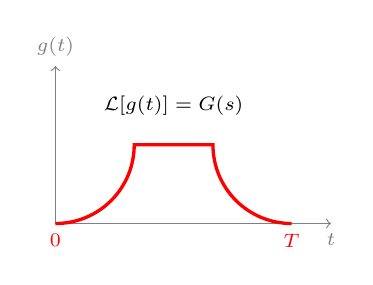
\begin{tikzpicture}
        \draw[->,gray] (0,0) -- (3.5,0) node[below] {\scriptsize$t$};
        \draw[->,gray] (0,0) -- (0,2) node[above] {\scriptsize$g(t)$};
        \draw[red,very thick] (0,0) node[below] {\scriptsize$0$} to [out=0,in=270] (1,1)
          -- (2,1) to [out=270,in=180] (3,0) node[below] {\scriptsize$T$};
        \node at (1.5,1.5) {\scriptsize$\mathcal{L}[g(t)]=G(s)$};
      \end{tikzpicture}
    \end{subfigure}
    \begin{subfigure}[b]{0.3\textwidth}
      \centering
      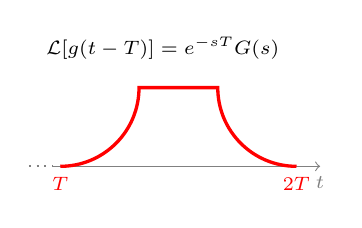
\begin{tikzpicture}
        \node at (1.5,1.5) {\scriptsize$\mathcal{L}[g(t-T)]=e^{-sT}G(s)$};
        \draw[dotted,gray,thick] (-.2,0)--(.1,0);
        \draw[->,gray] (.1,0) -- (3.5,0) node[below] {\scriptsize$t$};
        \draw[red,very thick] (0.2,0) node[below] {\scriptsize$T$} to [out=0,in=270] (1.2,1)
          -- (2.2,1) to [out=270,in=180] (3.2,0) node[below] {\scriptsize$2T$};
      \end{tikzpicture}
    \end{subfigure}
    \begin{subfigure}[b]{0.3\textwidth}
      \centering
      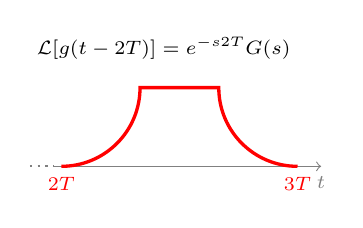
\begin{tikzpicture}
        \node at (1.5,1.5) {\scriptsize$\mathcal{L}[g(t-2T)]=e^{-s2T}G(s)$};
        \draw[dotted,gray,thick] (-.2,0)--(.1,0);
        \draw[->,gray] (.1,0) -- (3.5,0) node[below] {\scriptsize$t$};
        \draw[red,very thick] (0.2,0) node[below] {\scriptsize$2T$} to [out=0,in=270] (1.2,1)
          -- (2.2,1) to [out=270,in=180] (3.2,0) node[below] {\scriptsize$3T$};
      \end{tikzpicture}
    \end{subfigure}
    \caption{}
    \label{fig:ej_potencial}
  \end{figure}
  Entonces consideramos una función periódica $f(t)$ de periodo $T$, que coincide con $g(t)$ en el intervalo $0\leqslant t\leqslant T$.
  \begin{align*}
    \mathcal{L}[f(t)] &= G(s)+G(s)e^{-sT}+G(s)e^{-s2T} + G(s)e^{-s3T}+\dots \\ 
    F(s) &= G(s)[1+e^{-sT}+e^{-2sT}+e^{-3sT}+\dots]  
  \end{align*}
  En el corchete del segundo miembro, tenemos una serie geométrica de razón $r=e^{-sT}$ que cumple con la condición $r<1$, por lo tanto su suma es 
  $$
  F(s)=G(s)\cdot \frac{1}{1-e^{-sT}} = \frac{G(s)}{1-e^{-sT}}
  $$
  que es la transformada de una función de periodo $T$.
\end{example}

\subsection{Teorema del desplazamiento complejo}

\begin{theorem}
  Sea $\mathcal{L}[f](s)=F(s)$ para $s>b\geqslant0$. Sea $a$ cualquier numero. Entonces 
  $$
  \mathcal{L}[e^{at}f(t)](s)=F(s-a) \qquad \text{para } s>a+b 
  $$
\end{theorem}
\begin{proof}
  Calculamos 
  $$
  \mathcal{L}[e^{at}f(t)]= \int_0^\infty e^{at}e^{-st}f(t)dt = \int_0^\infty e^{-(s-a)t}f(t)dt = F(s-a)
  $$
  quedando demostrado.
\end{proof}

Si el desplazamiento fuera a la izquierda $F(s+a)=\mathcal{L}[f(t)e^{-at}$

\subsection{Teorema de la derivación compleja}

Buscamos la transformada de Laplace de una función que está multiplicada por $t$ o por una potencia de $t$. La integral en estos casos es más difícil de resolver, por eso se recurre al teorema.

\begin{theorem}
  El teorema establece
  $$
  \mathcal{L}[f(t)t]=-\frac{d}{ds}(F(s))
  $$
\end{theorem}
\begin{proof}
  Derivamos la expresión de la transformada respecto de $s$:
  $$
  \frac{d}{ds}\mathcal{L}[f(t)] = \int_0^\infty -t\cdot e^{-st}\cdot f(t)dt 
  $$
  Llamamos $g(t)=t\cdot f(t)$, 
  $$
  -\int_0^\infty g(t)e^{-st}dt = -G(s)
  $$
  donde $G(s)=F(t\cdot f(t))$. Entonces 
  $$
  \mathcal{L}[f(t)\cdot t] = (-1) \frac{d}{ds}F(s)
  $$
\end{proof}
Este teorema puede generalizarse para la potencia $n$-ésima, siendo:
$$
\mathcal{L}[f(t)\cdot t^n]=(-1)^n \frac{d^n}{ds^n}F(s)
$$

\subsection{Teorema de la convolución}

También llamado teorema de Duhamel\footnote{Jean-Marie Constant Duhamel fue un matemático y físico francés.} Establece lo siguiente. 
\begin{theorem}
  El teorema establece 
  $$
  \mathcal{L}[h(t)]=F_1(s)F_2(s)
  $$
  O en palabras: la transformada del producto de convolución de dos funciones del tiempo es igual al producto ordinario de las transformadas de Laplace de dichas funciones.
\end{theorem}

Antes de ver la demostración a este teorema se enuncia la definición de convolución de funciones.

\begin{definition}[Convolución]
  La convolución es una operación matemática que combina dos señales de entrada para producir una tercera señal. En el campo de las señales digitales es muy importante ya que permite obtener la salida de un sistema a partir de la señal de entrada y la respuesta al impulso.
  $$
  h(t)=f_1(t)\ast f_2 (t) =\int_0^t f_1(t-\tau) f_2(\tau) d\tau
  $$
\end{definition}

% Esta última parte no me gasté en lo absoluto. Necesito terminar de estudiar. Debe mejorarse todo este capítulo.

¿De donde surge esta integral?

Tomemos como ejemplo la función definida por
$$
f(t)=\begin{cases}
  E e^{-at} & \text{para } t\geqslant b \\ 
  0 & \text{para } 0 < t < ?
\end{cases}
$$
% Muchos gráficos. La demostración de esto está expuesta de una forma muy resumida y no lo logro entender. Hasta acá llegaré por ahora.
